\newpage
\section{Resultados: \textit{Market Share} e Cenários de Frota}
\label{sec:resultados}

% ===========================================================
\subsection{Market Share de Químicas de Baterias}
\label{sec:marketshare}
% ===========================================================

Determinar a participação de mercado (\textit{market share}) das diferentes
químicas de baterias em circulação no Brasil é uma etapa fundamental para
caracterizar a frota eletrificada e orientar a escolha da química do estudo
industrial. Para isso, o levantamento baseou-se no cruzamento de dados de
emplacamentos de veículos eletrificados, fornecidos pela Associação Brasileira do
Veículo Elétrico (ABVE), com as especificações técnicas do Programa Brasileiro de
Etiquetagem Veicular (PBEV), conforme descrito na Seção~\ref{sec:met-marketshare}.

A partir da consolidação desses dados, que englobou uma amostra de mais de
509~mil veículos eletrificados, foi possível estimar a participação de cada
tecnologia de bateria nos emplacamentos. As participações são calculadas em número
de veículos; por isso, refletem a frequência de cada química, e não sua
participação em massa ou em capacidade. Os resultados revelam uma configuração de
mercado particular, moldada pela predominância de modelos de entrada e híbridos.

A química de Lítio-Ferro-Fosfato (LFP) representa \textbf{48,12\%} dos veículos
analisados. Esse domínio reflete a forte penetração de montadoras asiáticas no
Brasil, que priorizam o LFP para reduzir o custo final ao consumidor e viabilizar
a comercialização de veículos elétricos e híbridos \textit{plug-in}.

Em segundo lugar, as baterias baseadas em Níquel-Manganês-Cobalto (NMC) respondem
por \textbf{32,75\%} da amostra. Sua aplicação concentra-se em veículos que
demandam maior densidade energética, como modelos de alta performance e híbridos
\textit{plug-in} de categorias superiores.

Destaca-se também a participação expressiva das baterias NiMH (níquel-metal
hidreto), que compõem \textbf{18,38\%} da amostra. Esse volume é sustentado quase
exclusivamente pelos híbridos convencionais (HEV) da Toyota. Tecnologias
minoritárias — NCMA (0,52\%), LMO/NMC (0,15\%) e variações de íon-lítio ainda em
confirmação (0,08\%) — somam juntas menos de 1\% do total, conforme sintetizado na
Tabela~\ref{tab:marketshare-sintese} e ilustrado na Figura~\ref{fig:marketshare}.

\begin{table}[H]
\centering
\caption{Síntese do \textit{market share} por química de bateria nos veículos
         eletrificados emplacados (participação em número de veículos).}
\label{tab:marketshare-sintese}
\begin{tabular}{lc}
\toprule
\textbf{Química da Bateria} & \textbf{Market Share} \\
\midrule
LFP (Lítio-Ferro-Fosfato)                          & 48,12\% \\
NMC (Níquel-Manganês-Cobalto)                      & 32,75\% \\
NiMH (Níquel-Metal Hidreto)                        & 18,38\% \\
NCMA (Níquel-Cobalto-Manganês-Alumínio)            &  0,52\% \\
LMO/NMC (Óxido de Manganês / Níquel-Mang.-Cobalto) &  0,15\% \\
Lítio-Íon (a confirmar)                            &  0,08\% \\
\bottomrule
\end{tabular}
\fonte{elaborada com base em \citeonline{ABVE} e \citeonline{PBEV}.}
\end{table}

\begin{figure}[H]
    \centering
    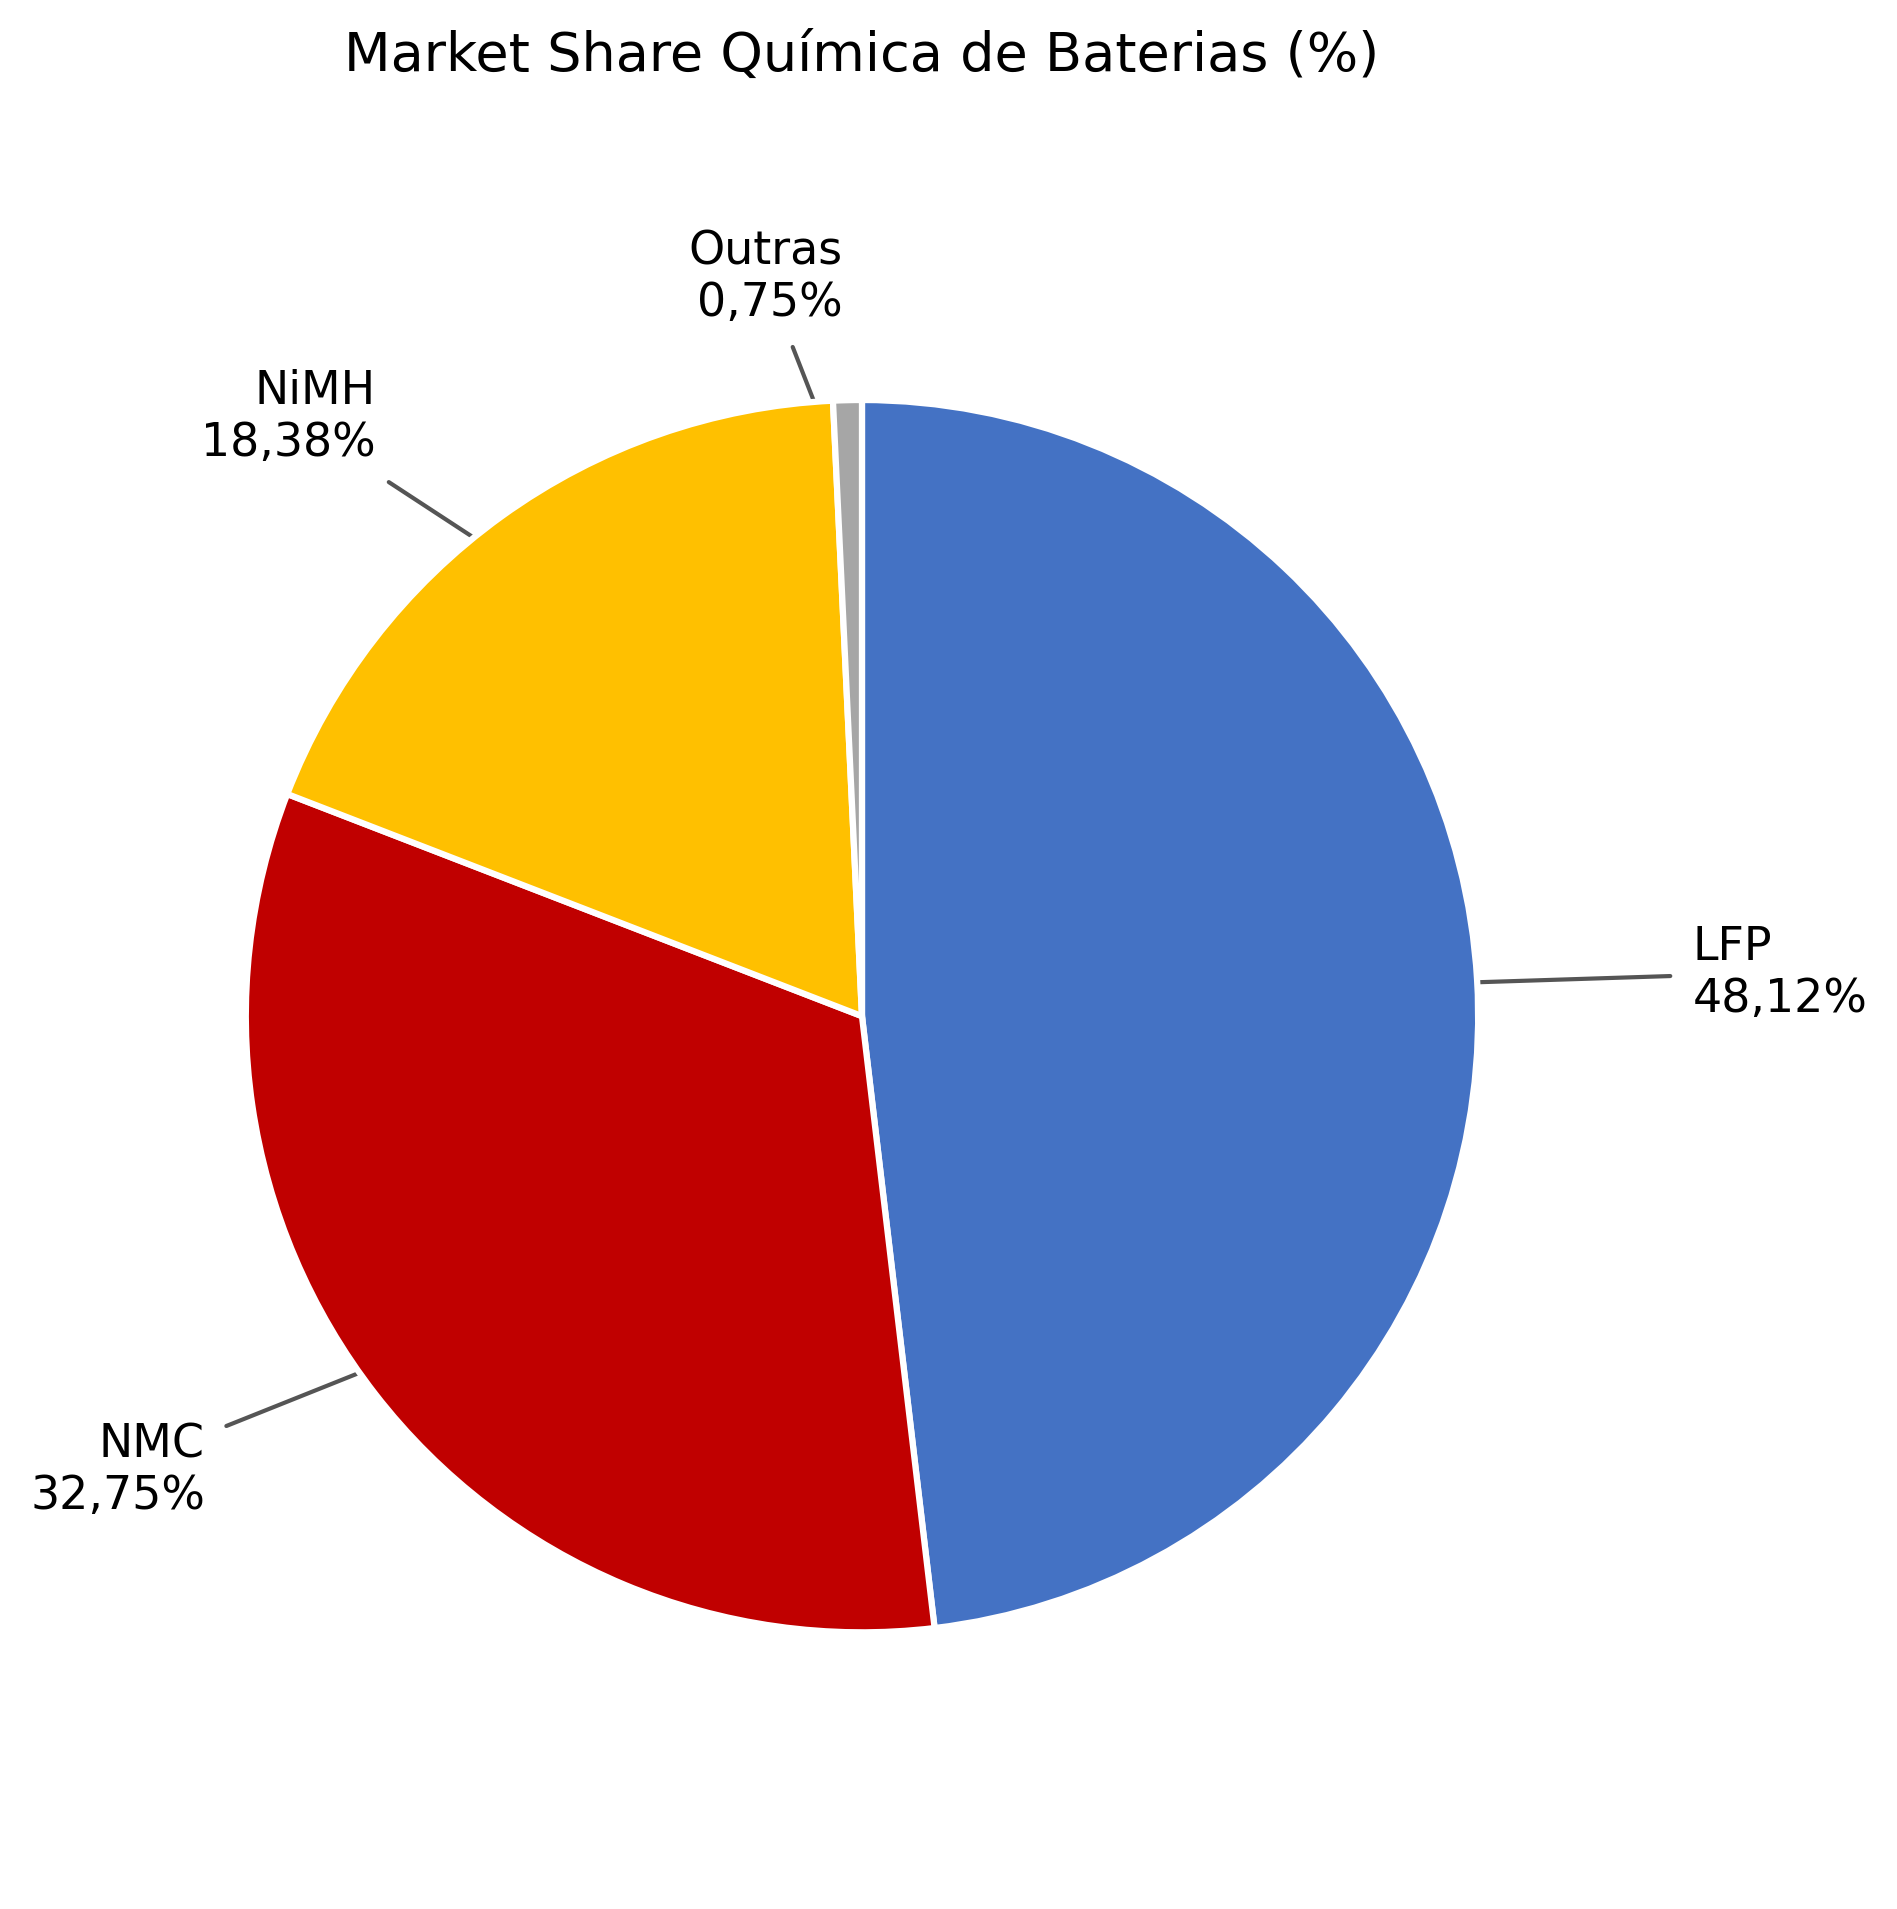
\includegraphics[width=0.6\textwidth]{figuras/market_share_quimicas.png}
    \caption{Participação das químicas de bateria nos veículos eletrificados
             emplacados (em número de veículos).}
    \label{fig:marketshare}
    \fonte{elaborada com base em \citeonline{ABVE} e \citeonline{PBEV}.}
\end{figure}

Este panorama estabelece a linha de base da composição química da frota
eletrificada. A predominância de químicas isentas de cobalto e níquel (como o LFP)
na maior parcela dos veículos indica que o futuro brasileiro terá uma concentração
expressiva de ferro, fósforo e lítio nas baterias em circulação, reforçando a
premissa de que a reciclagem no país exigirá processos eficientes, focados em
ganho de escala.

\subsubsection{Base de Dados de Emplacamentos}
\label{subsec:emplacamentos}

A Tabela~\ref{tab:emplacamentos-geral} apresenta os 15 modelos eletrificados de
maior volume de vendas (todas as categorias combinadas), com a química de bateria
atribuída a cada um. As participações por modelo são calculadas sobre o total de
emplacamentos da base — cerca de 593~mil veículos, valor implícito na própria
tabela (51.551 / 8,69\%) —, e não sobre a amostra de 509~mil veículos com química
identificada utilizada na Tabela~\ref{tab:marketshare-sintese}
\pendente{confirmar os dois denominadores na planilha-fonte e o número de modelos
da amostra geral: a nota da tabela cita 50 modelos, e as
Tabelas~\ref{tab:bev} e~\ref{tab:hev} listam 49 BEV e 21 HEV}.

\begin{table}[H]
\centering
\caption{Modelos eletrificados de maior volume de emplacamento (geral) e química
         de bateria associada.}
\label{tab:emplacamentos-geral}
\begin{tabular}{lccc}
\toprule
\textbf{Modelo} & \textbf{Quantidade} & \textbf{Market Share} & \textbf{Química} \\
\midrule
Toyota Corolla Cross XRX Hybrid & 51.551 & 8,69\% & NiMH \\
BYD Dolphin Mini GS5 EV         & 44.730 & 7,54\% & LFP \\
BYD Song Plus GS DM             & 44.652 & 7,53\% & LFP \\
BYD Dolphin GS 180 EV           & 32.334 & 5,45\% & LFP \\
BYD Song Pro GS DM              & 30.274 & 5,11\% & LFP \\
Toyota Corolla Altis Premium H  & 22.147 & 3,73\% & NiMH \\
GWM Haval H6 PHEV 19            & 16.946 & 2,86\% & NMC \\
BYD Dolphin Mini GS EV          & 15.820 & 2,67\% & LFP \\
GWM Haval H6 Premium HEV        & 15.623 & 2,63\% & NMC \\
BYD King GS DM                  & 15.181 & 2,56\% & LFP \\
GWM Haval H6 GT                 & 13.088 & 2,21\% & NMC \\
GWM Haval H6 Premium PHEV       & 10.911 & 1,84\% & NMC \\
CAOA Chery Tiggo 8 PHEV         &  9.759 & 1,65\% & NMC \\
BYD Seal AWD GS 590 EV          &  8.132 & 1,37\% & LFP \\
BYD Dolphin Plus 310 EV         &  7.631 & 1,29\% & LFP \\
\bottomrule
\end{tabular}
\fonte{elaborada com base em \citeonline{ABVE} e \citeonline{PBEV}.}
\end{table}

\subsubsection{Composição por Categoria de Veículo}
\label{subsec:composicao-categoria}

Segmentando a amostra por categoria de veículo, observa-se que a predominância do
LFP concentra-se nos modelos 100\% elétricos (BEV) — nove dos doze modelos da
Tabela~\ref{tab:bev} utilizam LFP —, enquanto o NiMH está associado quase
exclusivamente aos híbridos convencionais (HEV) da Toyota; o Honda Civic Hybrid
da amostra utiliza bateria de íon-lítio. Não foi possível isolar, na base de dados
consultada, uma quebra específica para a categoria de híbridos \textit{plug-in}
(PHEV): os modelos dessa categoria permanecem diluídos no levantamento agregado da
Tabela~\ref{tab:emplacamentos-geral} (por exemplo, GWM Haval H6 PHEV, CAOA Chery
Tiggo 8 PHEV e GWM Tank 300 PHEV), motivo pelo qual a segmentação apresentada a
seguir limita-se às categorias BEV e HEV.

\begin{table}[H]
\centering
\caption{Composição química — veículos 100\% elétricos (BEV), modelos mais
         relevantes.}
\label{tab:bev}
\begin{tabular}{lccc}
\toprule
\textbf{Modelo} & \textbf{Quantidade} & \textbf{Market Share (BEV)} & \textbf{Química} \\
\midrule
BYD Dolphin Mini GS5 EV  & 44.730 & 23,98\% & LFP \\
BYD Dolphin GS 180 EV    & 32.334 & 17,34\% & LFP \\
BYD Dolphin Mini GS EV   & 15.820 &  8,48\% & LFP \\
BYD Seal AWD GS 590 EV   &  8.132 &  4,36\% & LFP \\
BYD Dolphin Plus 310 EV  &  7.631 &  4,09\% & LFP \\
BYD Yuan Pro GS 290 EV   &  6.344 &  3,40\% & LFP \\
GWM Ora 03 Skin BEV48    &  5.780 &  3,10\% & LFP \\
BYD Yuan Plus GL 310 EV  &  5.390 &  2,89\% & LFP \\
GWM Ora 03 GT BEV63      &  4.305 &  2,31\% & NMC \\
Volvo EX30 E60 Ultra     &  3.275 &  1,76\% & NMC \\
Renault E-Kwid Intens    &  3.061 &  1,64\% & NMC \\
JAC E-JS1                &  2.872 &  1,54\% & LFP \\
\bottomrule
\end{tabular}
\fonte{elaborada com base em \citeonline{ABVE} e \citeonline{PBEV}. Amostra
       completa de 49 modelos (172.384 unidades, $\sim$92,4\% da categoria BEV).}
\end{table}

\begin{table}[H]
\centering
\caption{Composição química — híbridos convencionais (HEV), modelos mais
         relevantes.}
\label{tab:hev}
\begin{tabular}{lccc}
\toprule
\textbf{Modelo} & \textbf{Quantidade} & \textbf{Market Share (HEV)} & \textbf{Química} \\
\midrule
Toyota Corolla Cross XRX Hybrid & 51.551 & 34,91\% & NiMH \\
Toyota Corolla Altis Premium H  & 22.147 & 15,00\% & NiMH \\
GWM Haval H6 Premium HEV        & 15.623 & 10,58\% & NMC \\
Toyota RAV4 H SX AWD CNT        &  6.895 &  4,67\% & NiMH \\
GWM Haval H6 HEV                &  5.689 &  3,85\% & NMC \\
Toyota Corolla Cross XRV Hybrid &  5.367 &  3,63\% & NiMH \\
GWM Haval H6 HEV2               &  3.779 &  2,56\% & NMC \\
Toyota Corolla GLI HEV          &  3.503 &  2,37\% & NiMH \\
CAOA Chery Tiggo 7 Pro HA       &  3.340 &  2,26\% & NMC \\
Toyota Corolla Altis HV         &  3.298 &  2,23\% & NiMH \\
Honda Civic Hybrid Touring      &  3.265 &  2,21\% & Li-Ion (NMC) \\
\bottomrule
\end{tabular}
\fonte{elaborada com base em \citeonline{ABVE} e \citeonline{PBEV}. Amostra
       completa de 21 modelos (140.517 unidades, $\sim$95,1\% da categoria HEV).}
\end{table}

% ===========================================================
\subsection{Cenários de Frota}
\label{sec:cenarios-frota}
% ===========================================================

Para estabelecer as projeções de eletrificação da frota automotiva brasileira com
horizontes em 2030, 2035 e 2040, conforme descrito na
Seção~\ref{sec:met-cenarios}, foram sintetizadas as projeções de quatro fontes
institucionais: estudo ANFAVEA/BCG, PDE~2035 (EPE/MME), Bright Consulting e MBC
Brasil.

\subsubsection{Veículos Leves}
\label{subsec:leves}

Antes de discutir os cenários, é importante situar o peso de cada categoria na
massa de baterias, já que a análise de fluxo de materiais depende não apenas do
número de veículos, mas sobretudo da massa de bateria que cada categoria introduz
no sistema. A Tabela~\ref{tab:categoria-massa} combina o \textit{mix} de vendas de
eletrificados projetado pelo PDE~2035 para 2035 — 13\% HEV, 3,5\% PHEV e 6\% BEV
das vendas totais de veículos leves \cite{EPE2025}, ou 57,8\%, 15,6\% e 26,7\% das
vendas de eletrificados — com massas médias de pacote adotadas como hipótese.

\begin{table}[H]
\centering
\caption{Participação de cada categoria nas vendas de eletrificados (PDE~2035) e
         na massa de baterias vendidas.}
\label{tab:categoria-massa}
\small
\setlength{\tabcolsep}{5pt}
\begin{tabular}{lccc}
\toprule
\textbf{Categoria} & \textbf{Vendas de eletrificados} & \textbf{Massa média do pacote (H)} &
\textbf{Massa de baterias vendidas} \\
\midrule
HEV  & 57,8\% & $\sim$40\,kg  & 14,1\% \\
PHEV & 15,6\% & $\sim$130\,kg & 12,4\% \\
BEV  & 26,7\% & $\sim$450\,kg & 73,5\% \\
\bottomrule
\end{tabular}
\fonte{elaborada com base no \textit{mix} de vendas de \citeonline{EPE2025}; massas
       médias de pacote: hipótese deste trabalho \pendente{indicar a fonte das massas
       médias de pacote}.}
\end{table}

O contraste entre as colunas da Tabela~\ref{tab:categoria-massa} é revelador:
embora o HEV responda pela maior parte das vendas de eletrificados (57,8\%), sua
contribuição para a massa de baterias vendidas é pequena (14,1\%), dado o pacote
reduzido. Já o BEV, com pouco mais de um quarto das vendas, concentra cerca de
três quartos (73,5\%) da massa de bateria que entrará futuramente no fluxo de
reciclagem. A conclusão é robusta às massas adotadas: variações de $\pm$30\% na
massa média do pacote BEV mantêm sua participação entre 66\% e 78\%. Essa
constatação reforça a necessidade de tratar a análise de fluxo de materiais em
base mássica, e não apenas em número de veículos, sob pena de subestimar
sistematicamente a demanda por lítio e demais materiais críticos.

As projeções institucionais convergem para uma rota distinta das dos mercados
europeu e chinês, com prioridade à hibridização, sobretudo ao Híbrido-Flex
(Seção~\ref{subsec:contexto-brasil}). A Tabela~\ref{tab:projecoes-fontes}
consolida as projeções das quatro fontes analisadas.

\begin{table}[H]
\centering
\caption{Comparativo das projeções de eletrificação por fonte.}
\label{tab:projecoes-fontes}
\small
\renewcommand{\arraystretch}{1.2}
\setlength{\tabcolsep}{4pt}
\begin{tabularx}{\textwidth}{@{} >{\raggedright\arraybackslash}p{2.5cm} >{\raggedright\arraybackslash}p{1.7cm} >{\raggedright\arraybackslash}p{2.0cm} X X @{}}
\toprule
\textbf{Fonte} & \textbf{Horizonte} & \textbf{Métrica} &
\textbf{Dados projetados} & \textbf{Premissa principal} \\
\midrule
ANFAVEA/\allowbreak BCG & 2030--2040 & Frota circulante (leves) &
Eletrificados: 35\% (transição gradual) e 42\% (transição acelerada) em 2040;
detalhamento na Tabela~\ref{tab:bcg} &
Transição gradual com Híbrido-Flex \textit{vs.} transição acelerada com maior
penetração de \textit{plug-ins} \\
\addlinespace
Bright Consulting & 2030 & Frota circulante &
$\sim$9,8\% híbridos (HEV/PHEV); $\sim$1,9\% elétricos puros (BEV); total
eletrificado $\sim$6,5--7 milhões \pendente{conferir na fonte} &
Eletrificação total (BEV) limitada por custo e infraestrutura; aposta de massa no
Híbrido-Flex \\
\addlinespace
PDE 2035 & 2035 & Vendas (licenciamento) &
22,5--23\% de participação de mercado anual; \textit{mix}: 13\% HEV, 3,5\% PHEV,
6\% BEV &
Preferência por híbridos que aproveitam a infraestrutura de abastecimento
existente \\
\addlinespace
PDE 2035 & 2035 & Frota circulante &
3,7 milhões de veículos eletrificados (8\% da frota total) &
Renovação de frota lenta; combustão/flex ainda 87\% da frota
\pendente{conferir: 8\% + 87\% = 95\%} \\
\addlinespace
MBC Brasil & 2040 & Frota circulante &
17,4 milhões de veículos eletrificados (27\% da frota total); 72\% dos
eletrificados híbridos &
Crescimento exponencial (44$\times$ até 2040) \\
\bottomrule
\end{tabularx}
\fonte{elaborada com base em \citeonline{anfaveabcg2024},
       \citeonline{BrightConsulting}, \citeonline{EPE2025} e
       \citeonline{MBCBrasil}.}
\end{table}

O estudo ANFAVEA/BCG trabalha com dois cenários principais de eletrificação:
\textbf{transição gradual} (conservadora, com aposta no Híbrido-Flex) e
\textbf{transição acelerada} (otimista, com maior penetração de
\textit{plug-ins}). A Tabela~\ref{tab:bcg} detalha a projeção da frota de veículos
leves por motorização para os três horizontes analisados.

\begin{table}[H]
\centering
\caption{Projeção da frota de veículos leves por motorização — estudo
         ANFAVEA/BCG (milhões de veículos).}
\label{tab:bcg}
\small
\setlength{\tabcolsep}{4.5pt}
\begin{tabular}{llccccccc}
\toprule
\textbf{Ano} & \textbf{Cenário} & \textbf{Frota total} & \textbf{BEV} &
\textbf{PHEV} & \textbf{HEV} & \textbf{MHEV} & \textbf{ICE/Flex} &
\textbf{Eletrificados (\%)} \\
\midrule
\multirow{2}{*}{2030} & Gradual   & 52 & 1  & 1 & 1 & 2 & 48 & 9  \\
                      & Acelerada & 52 & 2  & 1 & 1 & 2 & 47 & 10 \\
\addlinespace
\multirow{2}{*}{2035} & Gradual   & 60 & 4  & 1 & 3 & 4 & 48 & 20 \\
                      & Acelerada & 60 & 5  & 1 & 4 & 4 & 44 & 25 \\
\addlinespace
\multirow{2}{*}{2040} & Gradual   & 71 & 9  & 2 & 7 & 8 & 48 & 35 \\
                      & Acelerada & 71 & 12 & 2 & 8 & 6 & 42 & 42 \\
\bottomrule
\end{tabular}
\fonte{\citeonline{anfaveabcg2024}. Valores arredondados ao milhão; por isso, a
       soma das categorias difere da frota total em até 2 milhões, exceto em 2040
       (transição gradual), em que as categorias somam 74 milhões para uma frota
       de 71 milhões \pendente{conferir no relatório completo ANFAVEA/BCG, que
       também deve ser citado para os valores de 2030 e 2035}.}
\end{table}

As Figuras~\ref{fig:comparacao-frotas} e~\ref{fig:composicao-frota} comparam,
respectivamente, os volumes absolutos e a composição percentual da frota projetada
por cada fonte, sempre no horizonte de cada projeção.

\begin{figure}[H]
\centering
\begin{tikzpicture}
\begin{axis}[
    ybar,
    bar width = 10pt,
    width  = 14.5cm,
    height = 7.2cm,
    symbolic x coords = {2030,2035,2040},
    xtick = data,
    enlarge x limits = 0.25,
    ymin = 0, ymax = 32,
    ylabel = {Frota eletrificada (milhões de veículos)},
    ylabel style = {font=\footnotesize},
    ticklabel style = {font=\footnotesize},
    ymajorgrids = true,
    grid style = {dotted, gray!40},
    axis x line* = bottom,
    axis y line* = left,
    nodes near coords,
    nodes near coords style = {font=\scriptsize},
    every node near coord/.append style = {/pgf/number format/use comma},
    legend style = {at={(0.5,-0.16)}, anchor=north, legend columns=3,
                    font=\footnotesize, draw=none, column sep=8pt},
    legend cell align = left,
]
\addplot[fill=gigaVerde!45, draw=black!60] coordinates {(2030,5) (2035,12) (2040,26)};
\addlegendentry{ANFAVEA/BCG — gradual}
\addplot[fill=gigaVerde, draw=black!60, postaction={pattern=north east lines, pattern color=white}] coordinates {(2030,6) (2035,14) (2040,28)};
\addlegendentry{ANFAVEA/BCG — acelerada}
\addplot[fill=gigaAzul!35, draw=black!60, postaction={pattern=dots, pattern color=black!60}] coordinates {(2035,3.7)};
\addlegendentry{PDE 2035}
\addplot[fill=gigaLaranja!55, draw=black!60, nodes near coords={6,5--7}] coordinates {(2030,6.75)};
\addlegendentry{Bright Consulting}
\addplot[fill=gigaRoxo!35, draw=black!60, postaction={pattern=crosshatch, pattern color=black!50}] coordinates {(2040,17.4)};
\addlegendentry{MBC Brasil}
\end{axis}
\end{tikzpicture}
\caption{Frota de veículos eletrificados projetada por fonte e horizonte (milhões
         de veículos). Os valores ANFAVEA/BCG incluem os híbridos leves (MHEV);
         sem eles, 3/4~milhões (2030), 8/10~milhões (2035) e 18/22~milhões (2040)
         nos cenários gradual/acelerado.}
\label{fig:comparacao-frotas}
\fonte{elaborada com base em \citeonline{anfaveabcg2024}, \citeonline{EPE2025},
       \citeonline{BrightConsulting} e \citeonline{MBCBrasil}.}
\end{figure}

\begin{figure}[H]
\centering
\begin{tikzpicture}
\begin{axis}[
    ybar stacked,
    bar width = 15pt,
    width  = 15cm,
    height = 7.8cm,
    symbolic x coords = {B30,G30,A30,P35,G35,A35,M40,G40,A40},
    xtick = data,
    xticklabels = {Bright (2030), Gradual (2030), Acelerada (2030),
                   PDE (2035), Gradual (2035), Acelerada (2035),
                   MBC (2040), Gradual (2040), Acelerada (2040)},
    x tick label style = {rotate=35, anchor=east, font=\scriptsize},
    ymin = 0, ymax = 100,
    ylabel = {Participação na frota (\%)},
    ylabel style = {font=\footnotesize},
    yticklabel style = {font=\footnotesize},
    ymajorgrids = true,
    grid style = {dotted, gray!40},
    axis x line* = bottom,
    axis y line* = left,
    enlarge x limits = 0.07,
    legend style = {at={(0.5,-0.42)}, anchor=north, legend columns=3,
                    font=\footnotesize, draw=none, column sep=8pt},
    legend cell align = left,
]
\addplot[fill=gigaVerde, draw=black!60] coordinates
  {(B30,1.9) (G30,1.9) (A30,3.8) (P35,0) (G35,6.7) (A35,8.6) (M40,7.6) (G40,12.2) (A40,17.1)};
\addlegendentry{BEV}
\addplot[fill=gigaLaranja!60, draw=black!60, postaction={pattern=north east lines, pattern color=black!45}] coordinates
  {(B30,9.8) (G30,3.8) (A30,3.8) (P35,0) (G35,6.7) (A35,8.6) (M40,19.4) (G40,12.2) (A40,14.3)};
\addlegendentry{HEV + PHEV}
\addplot[fill=gigaAzul!30, draw=black!60, postaction={pattern=dots, pattern color=black!55}] coordinates
  {(B30,0) (G30,3.8) (A30,3.8) (P35,0) (G35,6.7) (A35,6.9) (M40,0) (G40,10.8) (A40,8.6)};
\addlegendentry{MHEV}
\addplot[fill=gigaRoxo!30, draw=black!60, postaction={pattern=crosshatch, pattern color=black!45}] coordinates
  {(B30,0) (G30,0) (A30,0) (P35,8) (G35,0) (A35,0) (M40,0) (G40,0) (A40,0)};
\addlegendentry{Eletrificados sem detalhamento}
\addplot[fill=gray!25, draw=black!60] coordinates
  {(B30,88.3) (G30,90.6) (A30,88.7) (P35,92.0) (G35,80.0) (A35,75.9) (M40,73.0) (G40,64.9) (A40,60.0)};
\addlegendentry{Combustão e demais}
\end{axis}
\end{tikzpicture}
\caption{Composição da frota de veículos leves projetada por fonte, no horizonte
         de cada projeção (\%). Para ANFAVEA/BCG, participações calculadas sobre a
         soma das categorias publicadas; para PDE, Bright e MBC, a parcela de
         combustão é obtida por diferença.}
\label{fig:composicao-frota}
\fonte{elaborada com base em \citeonline{anfaveabcg2024}, \citeonline{EPE2025},
       \citeonline{BrightConsulting} e \citeonline{MBCBrasil}.}
\end{figure}

A predominância de veículos híbridos (HEV) e híbridos \textit{plug-in} (PHEV)
sugerida pelas fontes impacta diretamente o dimensionamento da massa de baterias:
como as baterias de híbridos são significativamente menores que as de BEVs
(Tabela~\ref{tab:categoria-massa}), a demanda por lítio e outros materiais
críticos por veículo será menor do que em um cenário de eletrificação pura. O
número de veículos elétricos na frota e a participação de BEVs e PHEVs são,
portanto, as variáveis mais relevantes para uma futura Análise de Fluxo de
Materiais da frota.

\subsubsection{Veículos Pesados}
\label{subsec:pesados}

Para o segmento de pesados, as fontes divergem do caminho da bateria pura,
apontando para soluções a gás e hibridização, com nichos específicos para
elétricos.

\paragraph{Ônibus.}
Existe uma dicotomia clara entre urbano e rodoviário. Nos \textbf{urbanos},
observa-se forte eletrificação via baterias (BEV), impulsionada por políticas
públicas como o Novo PAC, com projeção de 28\% das vendas em 2035. Nos
\textbf{rodoviários}, a eletrificação pura enfrenta barreiras de autonomia e
infraestrutura, sendo a tendência híbrida ou a gás natural. Estima-se, para 2035,
uma frota de 48,5~mil ônibus eletrificados, dos quais 43,5~mil puramente elétricos,
com foco urbano \pendente{indicar a fonte dos valores para ônibus}.

\paragraph{Caminhões.}
O diesel deve permanecer dominante: em 2040, caminhões a diesel ainda
representarão cerca de 85\% da frota e, em 2035, o diesel responderá por 94\% das
vendas \pendente{confirmar no PDE~2035 se os 94\% se referem à frota ou às vendas
e o ano representado na Figura~\ref{fig:frota-pesados}}. O biometano é apontado
pelo MBC Brasil como principal substituto do diesel, com potencial técnico para
substituir até 70\% do consumo \cite{MBCBrasil} — evidenciando que a bateria não
é a única solução de baixo carbono para o segmento de carga. A eletrificação via
bateria deve concentrar-se na ``última milha'' (entregas urbanas) e em caminhões
semileves e leves (19\% das vendas em 2035).

\begin{figure}[H]
    \centering
    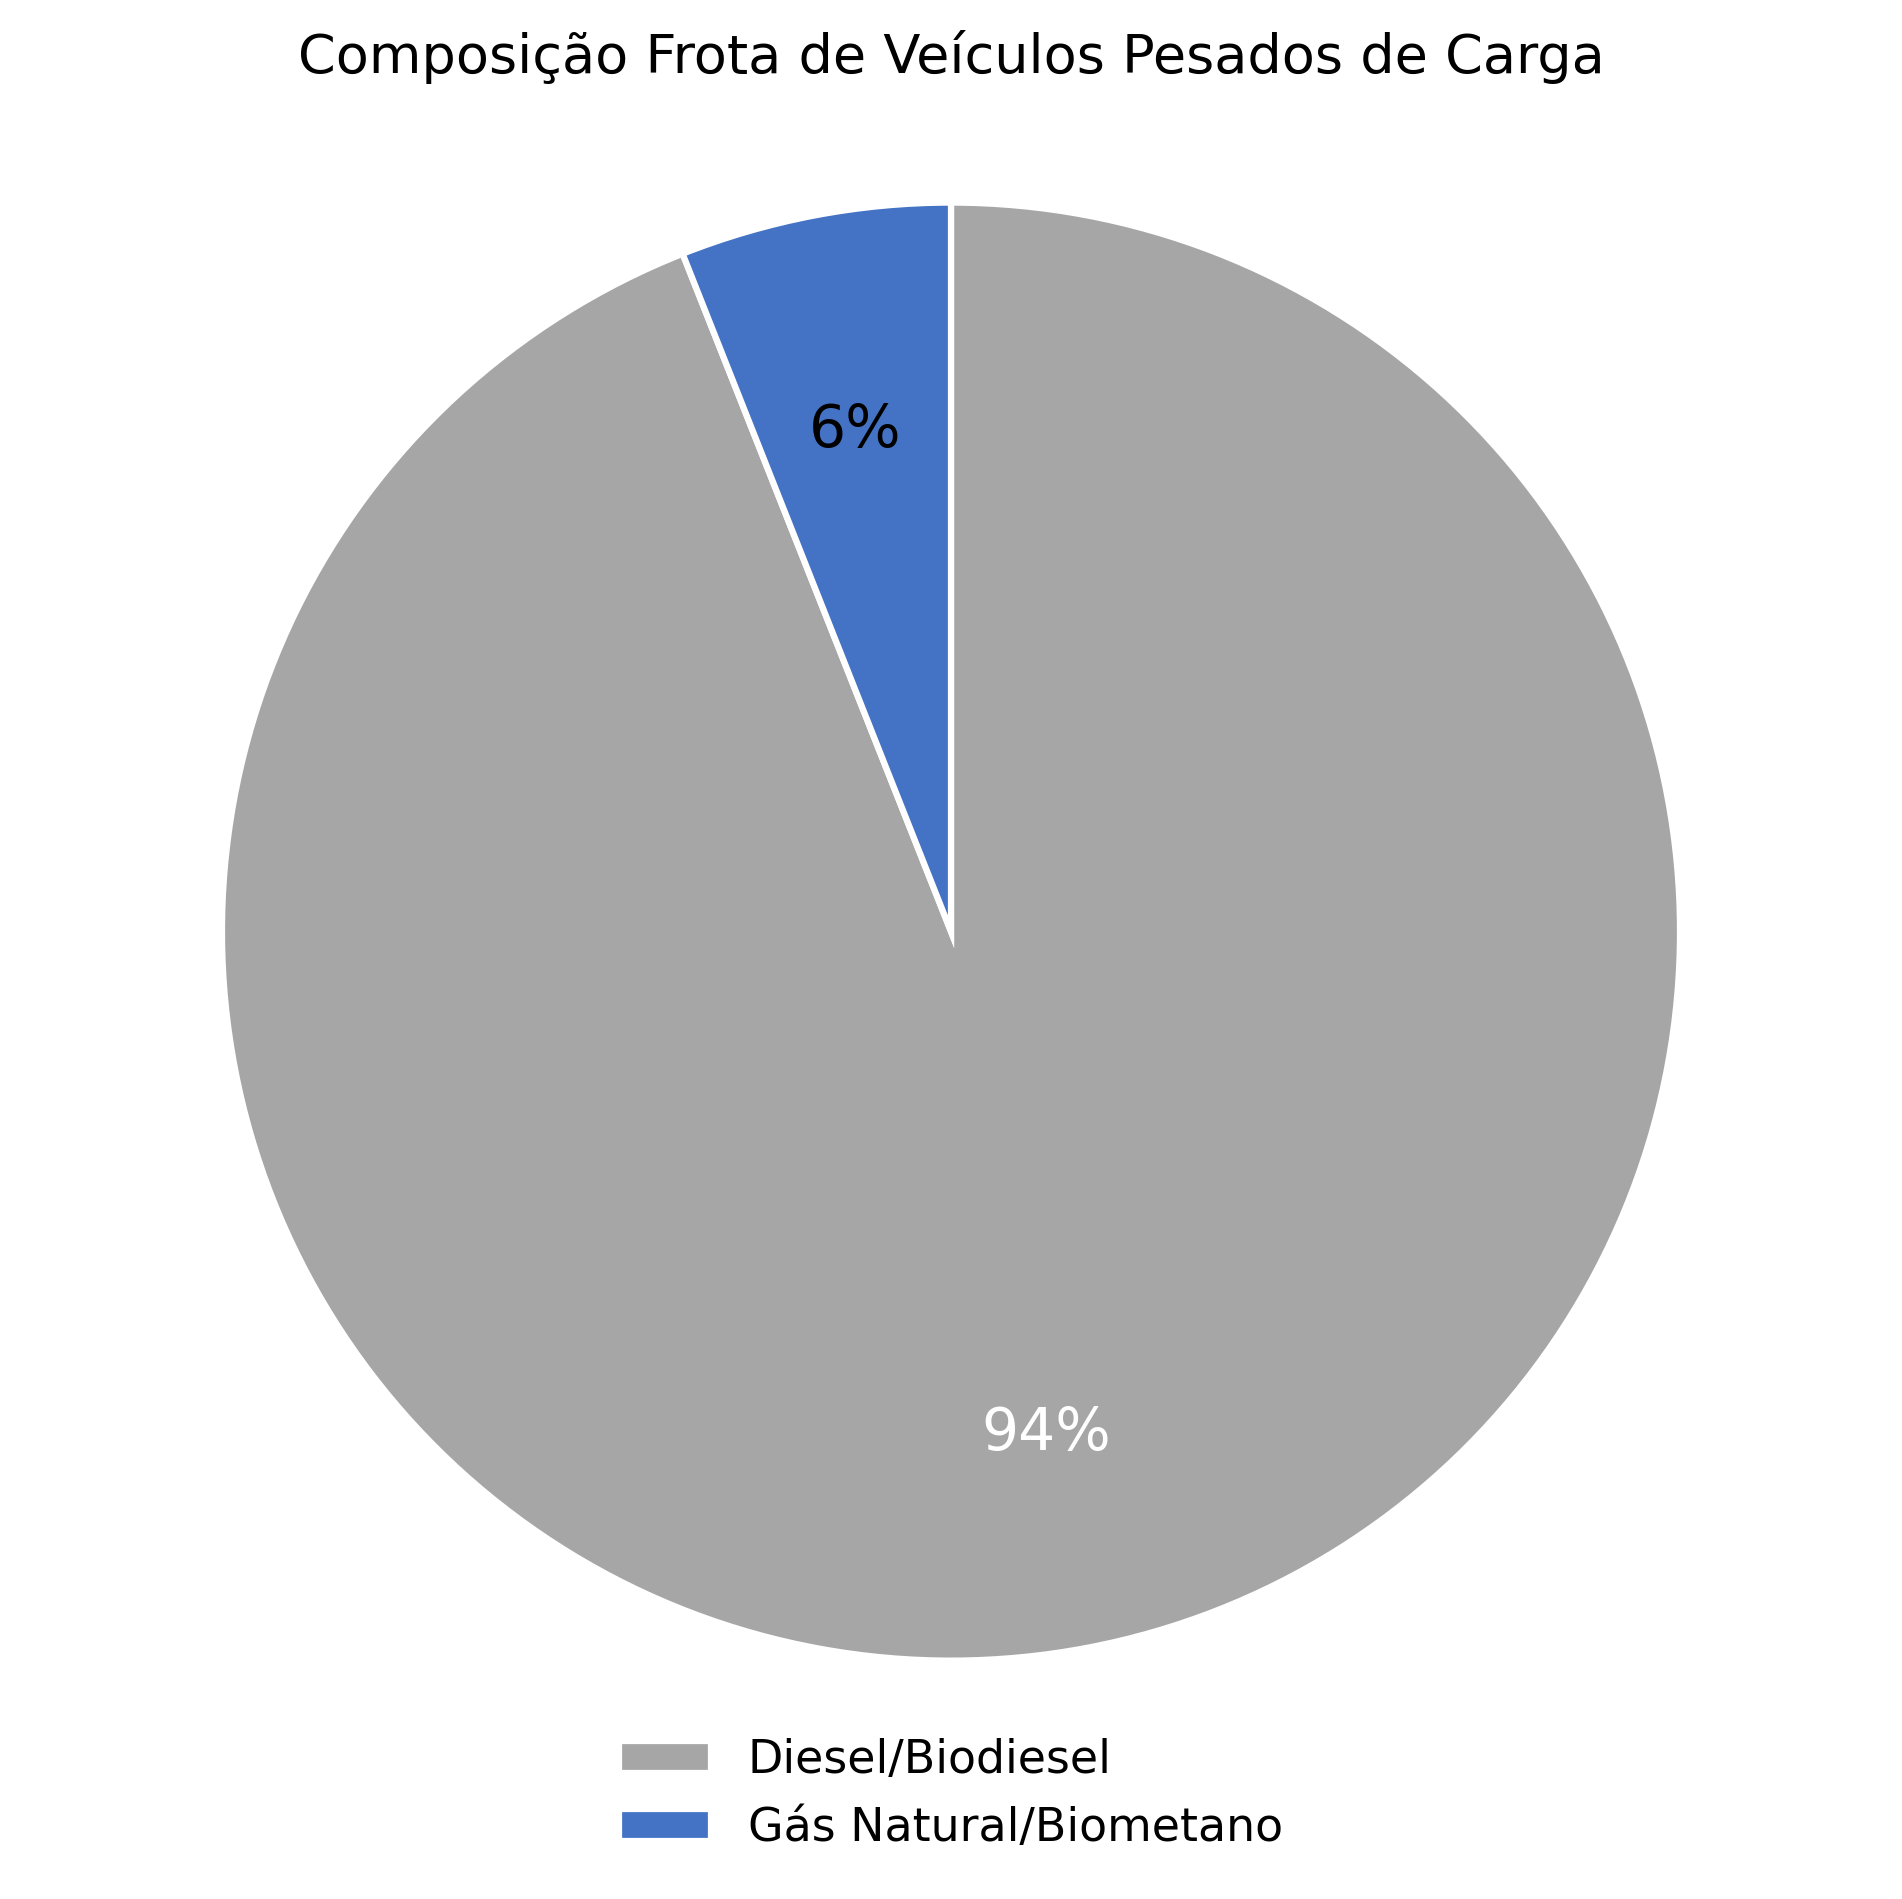
\includegraphics[width=0.55\textwidth]{figuras/frota_pesados_carga.png}
    \caption{Composição dos veículos pesados de carga por energético
             (diesel/biodiesel e gás natural/biometano).}
    \label{fig:frota-pesados}
    \fonte{elaborada com base em \citeonline{EPE2025}.}
\end{figure}

Diante da projeção de que apenas uma fração marginal ($\sim$2\%) da frota de
caminhões será composta por veículos elétricos \pendente{indicar a fonte do valor
de 2\%}, e da ausência de séries comparáveis às dos veículos leves para os ônibus,
os veículos pesados não integram os cenários quantitativos deste trabalho
(Seção~\ref{sec:met-cenarios}).

\subsubsection{Cenários Adotados}
\label{subsec:cenarios-sensibilidade}

Conforme a Seção~\ref{sec:met-cenarios}, os cenários \textbf{Conservador} e
\textbf{Acelerado} correspondem, respectivamente, aos cenários de transição
gradual e acelerada do estudo ANFAVEA/BCG. A
Tabela~\ref{tab:cenarios-adotados} resume as faixas resultantes para a frota
eletrificada de veículos leves.

\begin{table}[H]
\centering
\caption{Cenários de eletrificação da frota de veículos leves adotados neste
         trabalho (milhões de veículos).}
\label{tab:cenarios-adotados}
\small
\begin{tabular}{lcccccc}
\toprule
 & \multicolumn{2}{c}{\textbf{2030}} & \multicolumn{2}{c}{\textbf{2035}} &
   \multicolumn{2}{c}{\textbf{2040}} \\
\cmidrule(lr){2-3}\cmidrule(lr){4-5}\cmidrule(lr){6-7}
\textbf{Agregado} & \textbf{Cons.} & \textbf{Acel.} & \textbf{Cons.} &
\textbf{Acel.} & \textbf{Cons.} & \textbf{Acel.} \\
\midrule
Eletrificados, incluindo MHEV & 5 & 6 & 12 & 14 & 26 & 28 \\
Eletrificados, sem MHEV       & 3 & 4 &  8 & 10 & 18 & 22 \\
BEV + PHEV                    & 2 & 3 &  5 &  6 & 11 & 14 \\
\bottomrule
\end{tabular}
\fonte{elaborada com base na Tabela~\ref{tab:bcg} \cite{anfaveabcg2024}.}
\end{table}

Os dois cenários delimitam uma frota eletrificada de 5 a 6~milhões de veículos em
2030, de 12 a 14~milhões em 2035 e de 26 a 28~milhões em 2040, incluídos os
híbridos leves (MHEV); sem eles, de 3 a 4, de 8 a 10 e de 18 a 22~milhões. Para a
massa de baterias, os segmentos determinantes são o BEV e o PHEV
(Tabela~\ref{tab:categoria-massa}), que passam de 2--3~milhões em 2030 para
11--14~milhões em 2040.

A verificação cruzada com as demais fontes
(Figuras~\ref{fig:comparacao-frotas} e~\ref{fig:composicao-frota}) indica que:
(i)~a projeção da Bright Consulting para 2030 (6,5--7~milhões) situa-se acima de
ambos os cenários, mesmo com os MHEV; (ii)~a do PDE~2035 (3,7~milhões em 2035)
situa-se muito abaixo da faixa sem MHEV (8--10~milhões), refletindo a premissa de
renovação lenta da frota; e (iii)~a do MBC Brasil para 2040 (17,4~milhões) é
próxima do cenário Conservador sem MHEV (18~milhões). A faixa adotada é, portanto,
intermediária entre as projeções disponíveis, o que reforça seu uso como envelope
para análises futuras de demanda de materiais, mas depende da composição de cada
fonte, que nem sempre explicita a inclusão dos MHEV.

% ===========================================================
\subsection{Da Frota à Fábrica}
\label{sec:frota-fabrica}
% ===========================================================

Os resultados deste capítulo motivam o estudo industrial do
Capítulo~\ref{sec:gigafabrica} por três razões. Primeiro, o LFP é a química mais
frequente na amostra analisada (48,12\%) e predomina entre os BEV — nove dos doze
modelos da Tabela~\ref{tab:bev} —, categoria que concentra a maior parte da massa
de baterias (Tabela~\ref{tab:categoria-massa}). Segundo, ambos os cenários
projetam crescimento expressivo de BEV e PHEV, de 2--3~milhões em 2030 para
11--14~milhões de veículos em 2040 (Tabela~\ref{tab:cenarios-adotados}), o que
torna relevante compreender os fluxos de materiais e de energia da produção das
células que os equiparão. Terceiro, a fabricação de células gera, desde o início
da operação, um fluxo de material secundário homogêneo — a sucata de produção —,
que antecede os volumes de baterias pós-consumo e pode sustentar as primeiras
etapas de uma cadeia nacional de reciclagem
(Seção~\ref{subsec:sintese-reciclagem}).

O estudo industrial não modela a frota nem um conjunto de fábricas: quantifica os
fluxos por kWh de célula LFP e os normaliza para 1~GWh de produção anual. A
conversão dos cenários de frota em demanda anual de células, em GWh/ano, exigiria
capacidades médias de bateria por categoria e taxas de reposição, não levantadas
nesta etapa, e integra a continuidade do trabalho.
